\section{Relativistic Quantum Mechanics, Space-Time Coordinates}
\subsection{The Naive setup}
Let us discuss for a few minutes a subject that ``doesn't exist'' - we will see why through the discussion! Think of a quantum-mechanical particle with position $\v{X}$, momentum $\v{P}$, such that these follow the canonical commutation relations $[X_i, P_j] = i\hbar \delta_{ij}$. We will give this particle a relativistic expression for the energy:
\begin{equation}
    H = \sqrt{P^2c^2 + m^2c^4}
\end{equation}
We can now ask about this system. If we were naively trying to combine QM with SR, this would be the first kind of thing we would try. In this kind of system, we can discuss eigenstates of position and momentum (although of course these are not eigenstates in the true sense; they are not normalized):
\begin{equation}
    H\ket{p} = \sqrt{p^2c^2 + m^2c^4}\ket{p}
\end{equation}
the question of how this eigenstate evolves in time is a simple one; its a stationary state of the system, so only evolves according to some phase:
\begin{equation}
    \ket{p(t)} = e^{-\frac{i}{\hbar}Ht}\ket{p} = e^{-\frac{i}{\hbar}\sqrt{p^2c^2 + m^2c^4}t}\ket{p}.
\end{equation}
Of course nothing interesting happens to eigenstates of the Hamiltonian with time. The more interesting question is what would happen to an eigenstate of position? We can characterize this as the matrix element $bra{x_f}e^{-\frac{i}{\hbar}Ht}\ket{x_i}$ which is the probability (transition) amplitude that a particle starts at position $x_i$ and some time later is found at position $x_f$. From the above, we can calculate this as:
\begin{equation}
    \bra{x_f}e^{-\frac{i}{\hbar}Ht}\ket{x_i} = \int d^3p \braket{x_f}{p}e^{-\frac{i}{\hbar}\sqrt{p^2c^2 + m^2c^4}t}\braket{p}{x_i}
\end{equation}
Where we have inserted the resolution of the identity $\int d^3p \dyad{p}{p}$. The inner products of momentum and position we are familiar as:
\begin{equation}
    \braket{p}{x} = \frac{e^{-i\frac{\v{p}}{\hbar}\cdot\v{x}}}{(2\pi\hbar)^{3/2}}
\end{equation}
So then:
\begin{equation}
    \bra{x_f}e^{-\frac{i}{\hbar}Ht}\ket{x_i} = \int \frac{d^3p}{(2\pi\hbar)^3}e^{i\frac{\v{p}}{\hbar}\cdot(\v{x}_f - \v{x}_i) -\frac{i}{\hbar}\sqrt{p^2c^2 + m^2c^4}t}
\end{equation}
but this final expression we derive with the standard (naive) assumptions has problems. 

\subsection{Problem 1 - Lack of Lorentz Invariance}
For one, it is not Lorentz invariant. Why should an probability distribution change if we put the experiment on a train? Or if we put ourselves on a train and interpret the experiment? It transforms something like a charge density; the time component of a four-vector. This is because we have setup $\psi^\dag\psi$ to transform like the time-component of a four-vector, even though we want to normalize the wavefunction and this normalization should hold between all frames.

We could fix this up to be Lorentz invariant via an easy fix up; we insert a factor of the energy downstairs:
\begin{equation}
    \bra{x_f}e^{-\frac{i}{\hbar}Ht}\ket{x_i} = \int \frac{d^3p}{(2\pi\hbar)^3}\frac{mc^2}{\sqrt{pc^2 + m^2c^4}}e^{i\frac{\v{p}}{\hbar}\cdot(\v{x}_f - \v{x}_i) -\frac{i}{\hbar}\sqrt{p^2c^2 + m^2c^4}t}
\end{equation}
there is nothing in our theory that tells us why we do this, but it does work (and it will be something we get from QFT). When $pc^2 \ll m^2c^4$ (i.e. in the non-relativistic limit) the factor is one so we recover the NRQM result. Another note: inserting this factor has significant effects, where we have difficulty localizing the particle (this carries through to quantum field theory - we cannot localize a particle to a position smaller than its wavelength. But in NRQM we can do this; the wavefunction of a particle can be as sharply peaked as we need it to be).

\subsection{Problem 2 - Causality Violations}
The next problem is harder to patch up.

\begin{figure}[htbp]
    \centering
    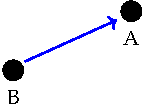
\includegraphics[]{Images/fig-RQMABcartoon.pdf}

    \caption{Consider an experiment where Bob releases a particle and Alice is some distance away. Under naive relativistic QM, Alice has a non-zero chance of measuring the particle to be at her position, even if she is so far away such that light would not be able to reach her in that time from when Bob released it.}
    \label{fig-RQMABcartoon}
\end{figure}
When we do the calculation for the probability of finding the particle some arbitrarily far distance away, we find that we have a non-zero probability regardless of the distance. To see this, let us return to the above transition probability. We can evaluate the integral approximately using the edge-of-the-wedge theorem. We note that $\bra{x_f}e^{-\frac{i}{\hbar}Ht}\ket{x_i}$ is analytic in the lower half of the complex time plane; this comes from the fact that that there the $ e^{-\frac{i}{\hbar}\sqrt{p^2c^2 + m^2c^4}t}$ leads to an exponential supression of the integral. As time comes to the real axis, it becomes much less nice (it becomes something like a distribution). We can define the value on the real axis as the limit taken from the analytic lower half time plane. How does this tell us anything? If the theory were causal, for small $t$ we would have to find that the integral is zero. But then we have some arc in the complex plane for which the function is zero. But if this region is in the region where the function is analytic, then by analytic continuation we could show that it would be zero everywhere. 

\begin{figure}[htbp]
    \centering
    \textcolor{blue}{Have: analyticity in the lower-half $t$ plane. In order for the theory to be causal, $t$ must be zero for small real $t$. But then we may use analytic continuation of the function to show that it is zero everywhere on the complex plane, since we have found an arc which it is zero on.}
    \caption{<caption>}
    \label{<label>}
\end{figure}


So the last step to show is that it is indeed analytic in this region. In the lower-$t$ plane, we can use Cauchy's integral formula to write:
\begin{equation}
    f(z_0) = \oint \frac{dz}{2\pi i}\frac{f(z)}{z - z_0}
\end{equation}
where $f = \bra{x_f}e^{-\frac{i}{\hbar}Ht}\ket{x_i}$ is our integral of interest. The value of the integral does not depend on the contour taken; let us deform the contour so that part of the contour lies on the real axis. We can then push the $z_0$ up until it is on the real axis; at this point the formula still holds, and so $f(z_0)$ is an analytic function on the real axis as well. Therefore by analytic continuation, the integral is zero everywhere. Contradiction!

\begin{figure}[htbp]
    \centering
    \textcolor{blue}{Contour integral + pushing it up}
    \caption{<caption>}
    \label{<label>}
\end{figure}

We therefore conclude that our theory violates causality. This would be ok if the universe actually behaved like this, but as far as we know we have never observed this; physics appears to be causal. So, this theory doesn't reflect reality, and we should throw it away.

\subsection{The QFT fix-up}

How does QFT fix this? First, we get the factor of $\frac{mc^2}{\sqrt{pc^2 + m^2c^4}}$ to preserve lorentz invariance. But the other thing we do is we make use of the negative energy branch of the energy spectrum:
\begin{equation}
    E = -\sqrt{p^2c^2 + m^2c^4}.
\end{equation}
When we calculate the same process in QFT, something gets added! We have two amplitudes:
\begin{equation}
    \bra{x_f}e^{-\frac{i}{\hbar}Ht}\ket{x_i} = \int \frac{d^3p}{(2\pi\hbar)^3}\left[\frac{mc^2}{\sqrt{pc^2 + m^2c^4}}e^{i\frac{\v{p}}{\hbar}\cdot(\v{x}_f - \v{x}_i) -\frac{i}{\hbar}\sqrt{p^2c^2 + m^2c^4}t} - \frac{mc^2}{\sqrt{pc^2 + m^2c^4}}e^{i\frac{\v{p}}{\hbar}\cdot(\v{x}_f - \v{x}_i) +\frac{i}{\hbar}\sqrt{p^2c^2 + m^2c^4}t}\right]
\end{equation}
i.e. we add a term that looks like time is running backwards. How do we interepret this? The first term/process has the interpretation of Bob having a particle and Alice detects it. The second term/process is as follows. When trying to detect a particle, Alice produces a particle-antiparticle pair, the antiparticle which goes the other direction and annhilates Bob's particle. We find in QFT that outside of the light cone that these two processes perfectly destructively interfere, and so causality is preserved!

An interesting note: if we repeated this analysis with a massless particle, we would find that the probability only has support on the lightcone (As we would expect; massless particles should travel on the lightcone!)

Another note: the addition of this second term destroys our analyticity argument as we now have one term that is analytic in the lower-$t$ plane and the other is analytic in the upper-$t$ plane. So we do not get the contradiction that the integral vanishes everywhere, as we did before.

Does this fixup fix everything? It seems to. They seem to be Lorentz invariant, and causal. This is why QFT gains the title of the natural marriage of quantum mechanics and special relativity (and string theory is known as the natural marriage of QM and GR - each are the only currently known solution to unifying these theories). Although this cannot be said of string theory yet, QFT at least seems to pass some very stringent experimental tests.

\subsection{Special Relativity and Minkowski Spacetime}
Once we go to a relativistic setting, it is natural to discuss space-time transformations (which are still translations, rotations and the like) which are symmetries of the space-time in which the QFT lives. We then try to write down the QFT such that these symmetries are not violated. We already know how to deal with this a little bit; we know Noether's theorem, and how to turn the crank and find conservation laws. We will therefore proceed to approach symmetries from a different point of view; as arising from the geometries of spacetime.

The space-time we consider is Minkowski spacetime; as much as we love curved spacetime, we won't consider it in this course here. It is described by coordinates:
\begin{equation}
    \v{x} = (x^1, x^2, x^3) \equiv x^a, \quad a = 1,2,3
\end{equation}
which describes three-dimensional infinite Euclidean space. The indices on the $x$s now have a position that means something. It is always up on a coordinate (or at least for the next while - $x_a$ is meaningless, for now). We will add to this another coordinate for time to make this a space-time (but we will give it units of distance to make it symmetric):
\begin{equation}
    x^0 \equiv ct
\end{equation}
where $x^0$ ranges over the real line. Combining these, we obtain a four-vector:
\begin{equation}
    x^\mu = (x^0, x^1, x^2, x^3), \quad \mu=0,1,2,3.
\end{equation}
We will generally use latin letters for regular vectors, and greek letters for four-vectors (though sometimes we leave it off entirely when the object is clear from context). The cartesian coordinates are not the only coordinates possible, but they are quite convenient; symmetries are quite apparent here.

\subsection{Coordinates on a space-time}
If we have a general spacetime, we could think about a coordinate system; all this would be is a dictionary for the various points in the spacetime, with points $x^\mu, y^\mu$ etc. There is of course a bunch of mathematical structure behind this, e.g. continuity/smoothness, this is done formally by locally mapping points (homeomorphism) to $\mathbb{R}^n$. We won't need this formality, but we will takeaway the idea of a coordinate transformation. Suppose we have a different coordinate system, with points $\tilde{x}^\mu, \tilde{y}^\mu$ etc. We could then compare dictionaries and figure out how to translate in between them. We could then define a transformation in between them: $\tilde{x}^\mu(x^\mu)$. This is a mathematical way of writing down a transformation, and the transformation inherits the ``smoothness'' of the coordinates (it is differentiable, invertible...). Formally, the invertiblity criterion is:
\begin{equation}
    \det(\frac{\partial }{\partial x^\mu}\tilde{x}^\nu) \neq 0.
\end{equation}

\subsection{Scalar Fields}
We consider a scalar field $\varphi(x^\mu)$; this is a physical entity that takes a value at each point in spacetime (for example; the temperature in a room). If someone else comes along with a different set of coordinates, we should agree with the value of the scalar field; so we should agree that:
\begin{equation}
    \varphi(x) = \tilde{\varphi}(\tilde{x})
\end{equation}
so a scalar field is defined in this way; with how it undergoes coordinate transformations.

We will discuss next time, but we can consider that displacement transforms like:
\begin{equation}
    dx^\nu = \frac{\partial x^\mu}{\partial \tilde{x}^\nu}d\tilde{x}^\nu
\end{equation}
So perhaps a vector field transforms in the same way:
\begin{equation}
    A^\mu(x) = \frac{\partial x^\mu}{\partial \tilde{x}^\nu} d\tilde{A}^\nu(x)
\end{equation}